% Created 2023-08-30 Wed 20:19
% Intended LaTeX compiler: pdflatex
\documentclass[stu, a4paper, 11pt, floatsintext]{apa7}
\usepackage[utf8]{inputenc}
\usepackage[T1]{fontenc}
\usepackage[ngerman]{babel}
\usepackage{graphicx}
\usepackage{longtable}
\usepackage{wrapfig}
\usepackage{rotating}
\usepackage[normalem]{ulem}
\usepackage{capt-of}
\usepackage{hyperref}

\title{Ausarbeitung Programiersprachen II: Autonomous Instantdocument System}
\shorttitle{Autonomous Instantdocument System}
\leftheader{Schwind}
\authorsnames{Jonas Schwind, Martin Boschmann}
\affiliation{Technische Hochschule Ostwestfahlen-Lippe}
\course{PGR2 8512: Programmiersprachen II}
\professor{Prof.\ Dr.\ rer.\ nat.\ Stefan Wolf}
\duedate{08.09.2023}

\hypersetup{
 pdfauthor={Jonas Schwind, Martin Boschman},
 pdftitle={Ausarbeitung Programiersprachen II},
 pdfkeywords={},
 pdfsubject={},
 pdfcreator={Emacs 27.1 (Org mode 9.6.1)}, 
 pdflang={English}}
\begin{document}

\maketitle
\tableofcontents
\clearpage
\listoffigures
\clearpage
\listoftables
\clearpage

\section{Analyse}
\subsection{Anforderungen}

\subsubsection{Erforderlich}

\begin{itemize}
\item Das Programm soll aus vorgefertigten (anpassbaren) Schnipseln ein \LaTeX{}-dokument erstellen.
\item Die Schnipssel werden in einer MySQL Datenbank verwaltet, diese soll sich zu einer CSV datei exportieren lassen.
\item Andere Einstellungen sollen in einer JSON verwaltet werden.
\item Die Konfigurationsdateien (Schnipsel eigeschlossen) sollen an dem Ort gespeichert werden, der vom Betriebssystem für diesen Zweck vogesehen ist.
\item Es soll eine Grafische Oberfläche für den gemeinen Nutzer, und eine CLI-Schnittstelle geben. Letztere emöglicht z.b. eine Automatisierung via cron.
\item Es soll eine Detailierte Anwenderdokumentation geben, welche auf github.com und in Form einer manpage (oder funktional vergleichbares) einsehbar ist.
\end{itemize}

\subsubsection{Optional}

\begin{itemize}
\item Das Programm sollte universell einsetzbar sein.
Das beduetet dass das Programm nicht zwingend für Klausuren eingesetzt werden muss, und auch für andere Dokumente verwendet werden kann.
\item \sout{Generierung neuer Schnippsel durch ChatGPT} (verworfen)
\end{itemize}

\subsection{Architektur}

\begin{figure}[!htbp]
\centering
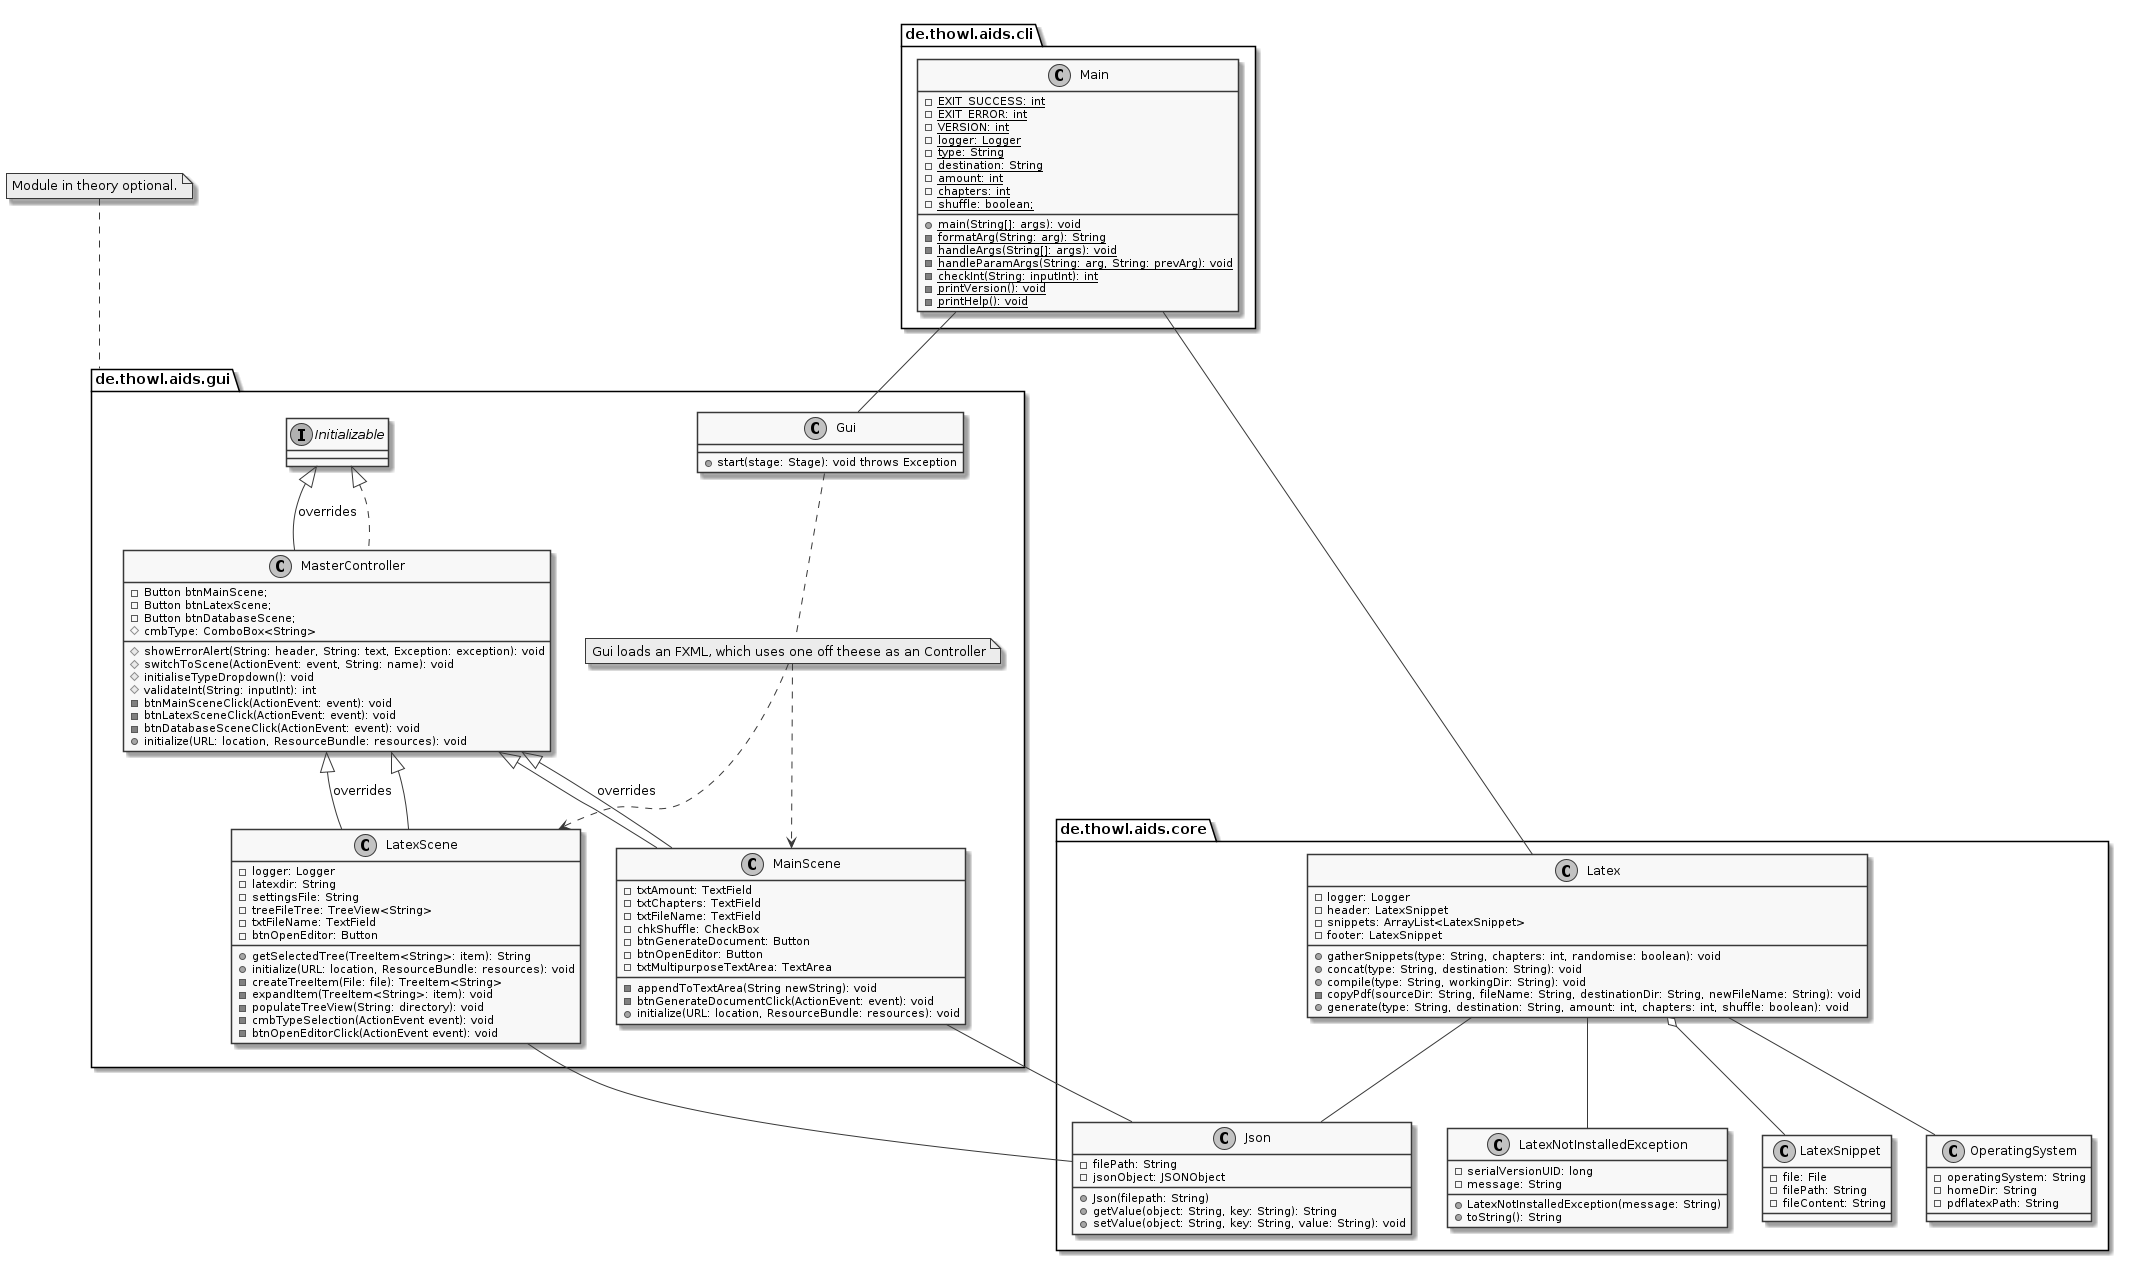
\includegraphics[width=.9\linewidth]{../technical_documentation/diagramm/uml/aids.png}
\caption{\label{Gesammtarchitektur}Gesammtarchitektur des Programms}
\end{figure}
\noindent Die Software ist modular aufgebaut. Das Projekt besteht aus 5 Modulen, davon sind 4 funktional und dienen der Umsetzung von Projektteilaspekten.
Das letzte Modul (welches hier nur als Modul bezeichnet wird, weil es von Maven als solches behandelt wird), dient als Sammelstelle für Dateien, die für eine Installation notwendig sind.

Der Zweck des modularen Aufbaus ist darin begründet, dass so jedem Teammitglied Module nach Bedarf zugewiesen werden können, und so die Verantwortlichkeiten geklärt werden.
Das in Abbildung~\ref{Gesammtarchitektur} gezeigte UML-Diagramm, zeigt die Softwarearchitektur des Projekts, die getter uns setter wurden hier und im folgenden jedoch nicht aufgeführt.

\subsection{Werkzeuge}
\noindent Im Folgenden wird eine Liste von Werkzeugen aufgeführt, die während der Entwicklung eingesetzt wurden.

\subsubsection{Entwicklungsumgebungen}
\begin{enumerate}
\item DOOM Emacs

DOOM Emacs ist eine Distribution von Emacs.
Es bietet einige vorkonfigurierte Pakete und Shortcuts, die das Programmieren erleichtern.

\item VS Code

VS Code ist ein Open-Source Code-Editor von Microsoft,
welcher mit einem Plugin auch die Programmierung in Java ermöglicht.
\end{enumerate}

\subsubsection{git}
\noindent git ist ein gängiges Versionskontrollsystem.
Es ermöglicht die Zusammenarbeit von mehreren Entwicklern am selben Projekt.

\subsubsection{JSON}
\noindent Javascript Objekt Notation (JSON) ist ein Datenformat welches wir dazu verwenden,
Einstellungen des Programms persistent zu halten.
Die Einstellungen werden in einer Datei gespeichert und bei Bedarf geladen.

\subsubsection{Maven}
\noindent Maven ist ein Build-Management-Tool für Java.
Es automatisiert das Verwalten von externen Libraries, das Compilieren des Codes,
und das Testen mit Unittests.

\subsubsection{plantuml}
\noindent plantuml ist ein textbasiertes Werkzeug zur Erstellung von UML-Diagrammen.
Die Diagramme werden mit einer Syntax definiert, die sich leicht in Quellcode übertragen lässt.

\subsection{Benutzerschnittstellen}

\subsubsection{CLI}
\noindent Es wurden folgende Argumente für die CLI-Schnittstelle festgelegt.

\begin{table}[htpb]
\centering
\caption{\label{argumente}CLI-Argumente}
\begin{tabular}{ll}
\toprule
Argument & Funktion \\
\midrule
\-t, --type <type> & Legt den Dokumenttyp fest.\\
-c, --chapters <chapters> & Legt die Kaptielanzahl pro Dokument fest.\\
-a, --amount <amount> & Legt die Anzahl der DokumentInstanzen fest.\\
-s, --shuffle & Schaltet den Shuffle modus an.\\
-h, --help & Zeigt eine Hilfe an.\\
-v, --version & Zeigt die versionsnummer an.\\
\bottomrule
\end{tabular}
\end{table}

\noindent Die in Tabelle~\ref{argumente} aufgeführten Argumente können auch in der Anwenderdokumentation nachgelesen werden.

\subsubsection{GUI}

TODO: .jpg einfügen

\clearpage

\section{Entwurf}

\subsection{de.thowl.aids.cli}

\noindent Das Modul \texttt{cli} ist der Startpunkt des Programms, es ist der CLI-Client oder startet die grafische Oberfläche. (s. Abbildung~\ref{CLI Architektur})

\begin{figure}[!htbp]
\centering
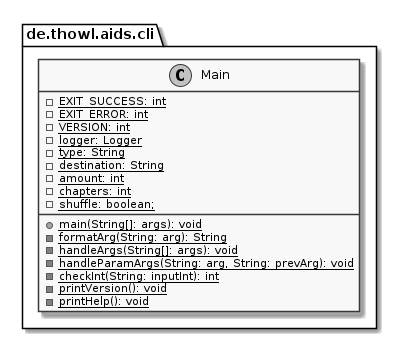
\includegraphics[width=250px]{../technical_documentation/diagramm/uml/flowcharts/cli/cli.png}
\caption{\label{CLI Architektur}Architektur des cli Moduls}
\end{figure}

\subsubsection{de.thowl.aids.cli.Main}
\noindent Die \texttt{main} Methode verwaltet die CLI-Argumente, sofern welche übergeben wurden.
Wenn keine Argumente übergeben wurden, startet das Programm mit einer grafischen Oberfläche.

Sollten Argumente übergeben worden sein, werden diese zunächst formatiert (s.
Abbildung\ref{formatArg-methode}). Im Anschluss werden die Argumente mit der  \texttt{handleArgs} Methode
abgearbeitet, sofern diese der Methode bekannt sind. (s.  Abbildung~\ref{handleArgs-methode})
Wenn \texttt{handleArgs} mit diesem Argument nichts anfangen kann, wird davon
ausgegangen, dass es sich bei diesem Argument um ein \emph{parametrisiertes Argument} handelt,
bspw. \texttt{–amount 10}. Diese werden von der \texttt{handleParamArgs} Methode verarbeitet (s.
Abbildung\ref{handleParamArgs-methode}).

\begin{figure}[!htbp]
\centering
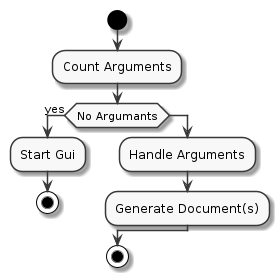
\includegraphics[width=150px]{../technical_documentation/diagramm/uml/flowcharts/cli/Main.png}
\caption{\label{main-methode}Ablaufdiagramm der main Methode}
\end{figure}

\begin{figure}[!htbp]
\centering
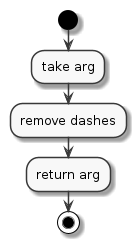
\includegraphics[width=150px]{../technical_documentation/diagramm/uml/flowcharts/cli/formatArg.png}
\caption{\label{formatArg-methode}Ablaufdiagramm der formatArg Methode}
\end{figure}

\begin{figure}[!htbp]
\centering
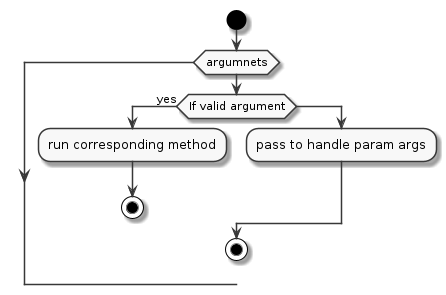
\includegraphics[width=150px]{../technical_documentation/diagramm/uml/flowcharts/cli/handleArgs.png}
\caption{\label{handleArgs-methode}Ablaufdiagramm der handleArgs Methode}
\end{figure}

\begin{figure}[!htbp]
\centering
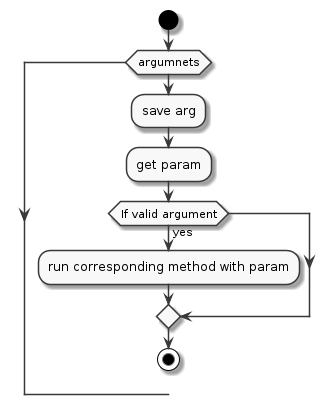
\includegraphics[width=150px]{../technical_documentation/diagramm/uml/flowcharts/cli/handleParamArgs.png}
\caption{\label{handleParamArgs-methode}Ablaufdiagramm der handleParamArgs Methode}
\end{figure}

\subsection{de.thowl.aids.core}
\noindent Im Modul \texttt{Core} sind alle essenziellen Klassen und Methoden vorhanden.
Es ist das Herzstück des Programms.

\begin{figure}[!htbp]
\centering
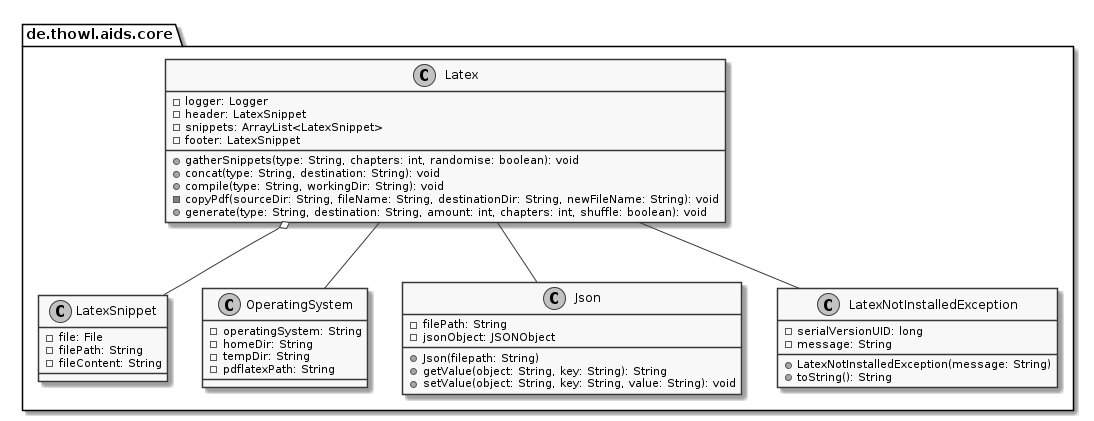
\includegraphics[width=350px]{../technical_documentation/diagramm/uml/flowcharts/core/core.png}
\caption{\label{Core Architektur}Architektur des core Moduls}
\end{figure}

\subsubsection{de.thowl.aids.core.Json}
\noindent Die \texttt{json} Klasse kümmert sich, wie der Name vermuten lässt, um die Datenhaltung/Verwaltung via JSON.

Die Ablaufdiagramme in Abbildung~\ref{getValue-methode} und Abbildung~\ref{setValue-methode} sind trivial und sprechen für sich selbst.

\begin{figure}[!htbp]
\centering
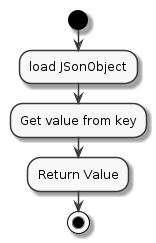
\includegraphics[width=150px]{../technical_documentation/diagramm/uml/flowcharts/core/json/getValue.png}
\caption{\label{getValue-methode}Ablaufdiagramm der getValue Methode}
\end{figure}

\begin{figure}[!htbp]
\centering
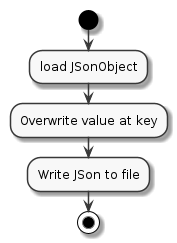
\includegraphics[width=150px]{../technical_documentation/diagramm/uml/flowcharts/core/json/setValue.png}
\caption{\label{setValue-methode}Ablaufdiagramm der setValue Methode}
\end{figure}

\subsubsection{de.thowl.aids.core.Latex}
\noindent  Die Klasse \texttt{Latex} dient zur Erstellung und Kompilierung von \LaTeX{} Dokumenten.

Die Methode \texttt{gatherSnippets} sammelt alle Schnipsel, die für ein \LaTeX{}-dokument benötigt werden.
Der Dokumentheader und Footer werden in je einer separaten Variable gespeichert (s. Abbildung~\ref{gatherSnippets-methode}).

Alle anderen Schnipsel landen in einer ArrayList.

Die Methode \texttt{concat} verbindet alle Schnippel, die von \texttt{gatherSnippets} gesammelt wurden, zu einer \texttt{.tex}-datei.
Der Inhalt des Headers und des Footers werden in die Datei kopiert.

Bei allen anderen Schnipseln wird der Dateipfad zu einem \texttt{\textbackslash{}inculde\{\}}
formatiert und eingefügt (s. Abbildung~\ref{concat-methode}).

Die \texttt{compile} Methode compiliert die von \texttt{concat} erstellte \LaTeX{}-datei zu einem PDF-Dokument (s. Abbildung~\ref{concat-methode}).

\begin{figure}[!htbp]
\centering
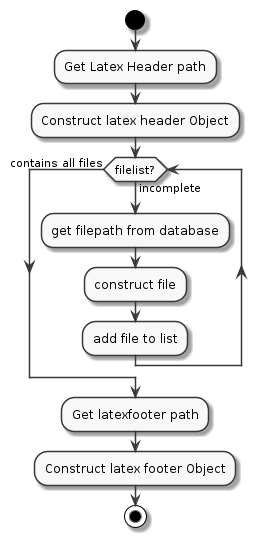
\includegraphics[width=150px]{../technical_documentation/diagramm/uml/flowcharts/core/latex/gatherSnippets.png}
\caption{\label{gatherSnippets-methode}Ablaufdiagramm der gatherSnippets Methode}
\end{figure}

\begin{figure}[!htbp]
\centering
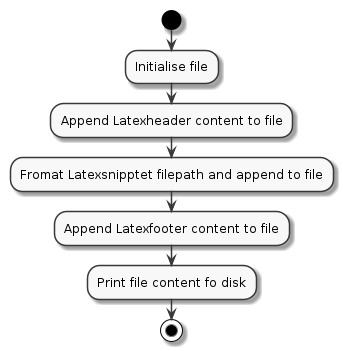
\includegraphics[width=150px]{../technical_documentation/diagramm/uml/flowcharts/core/latex/concat.png}
\caption{\label{concat-methode}Ablaufdiagramm der concat Methode}
\end{figure}

\begin{figure}[!htbp]
\centering
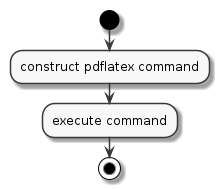
\includegraphics[width=150px]{../technical_documentation/diagramm/uml/flowcharts/core/latex/compile.png}
\caption{\label{compile-methode}Ablaufdiagramm der compile Methode}
\end{figure}

\subsubsection{de.thowl.aids.core.OperartingSystem}
\noindent Der in Abbildung~\ref{os-construcktor} visualisierte Konstruktor, legt die Objektattribute abhängig vom verwendetem Betriebssystem an.

Es soll vermieden werden, für das Programm wichtige Dateien sinnlos im Dokumente-Verzeichnis abzulegen. Daher werden die Dateipfade, die vom OS für diesen Zweck vorgesehen sind, verwendet.

Aus persönlichen Gründen kann die Verwendung unter macOS allerdings nicht getestet werden.

\begin{figure}[!htbp]
\centering
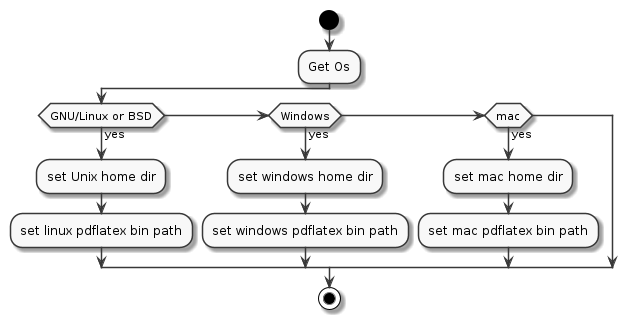
\includegraphics[width=250px]{../technical_documentation/diagramm/uml/flowcharts/core/os/construcktor.png}
\caption{\label{os-construcktor}Ablaufdiagramm des Konstrucktors der Klasse OperartingSystem}
\end{figure}

\subsection{de.thowl.aids.gui}
\noindent Das \texttt{gui} Modul ist für die grafische Oberfläche zuständig.
In diesem Abschnitt werebn Eventhandler nicht Betrachtet.

\begin{figure}[!htbp]
\centering
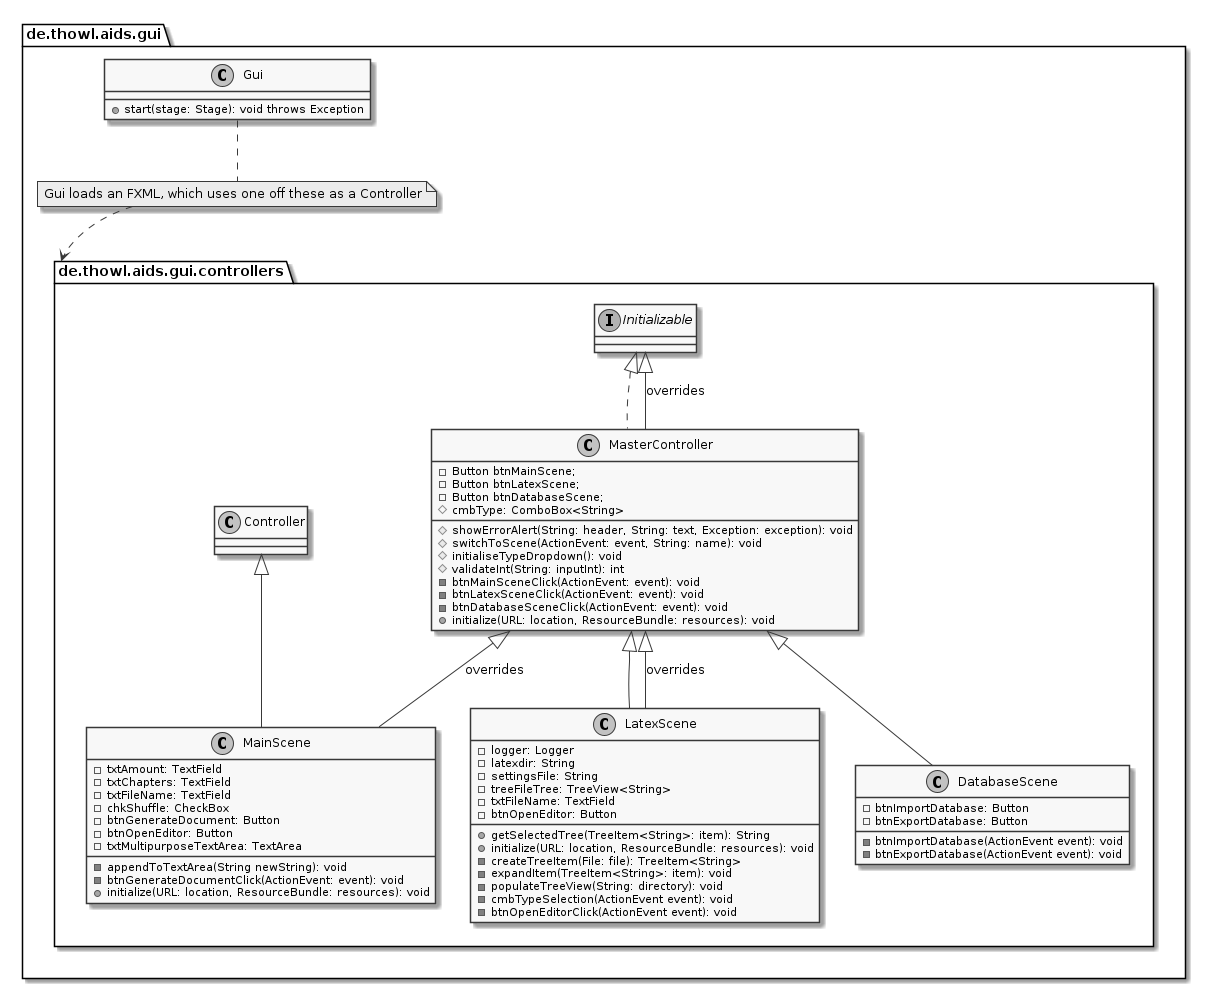
\includegraphics[width=350px]{../technical_documentation/diagramm/uml/flowcharts/gui/gui.png}
\caption{\label{gui Architektur}Architektur des gui Moduls}
\end{figure}

\subsection{de.thowl.aids.database}
\noindent Das \texttt{database} Modul ist für die Datenbank zuständig.

\subsubsection{de.thowl.aids.gui.Controller}
\noindent Die Klasse \texttt{Controller} ist eine abstrakte Klasse, von der alle GUI-Controller erben.

Die in Abbildung~\ref{initializeTypeDropdown-methode} dargestellte Methode füllt das TypeDropdown, welches dazu verwendet wird, den Dokumenttypen grafisch auszuwählen, mit Daten.
Der einfachste Weg dies zum Zeitpunkt der Implementierung zu realisieren ist es, die Dateistruktur im config-verzeichnis nachzubilden (s. Abbildung~\ref{initializeTypeDropdown-methode}).

Die \texttt{switchToScene} methode (Abbildung~\ref{switchToScene-methode}) wechselt die Szene in der GUI.
Dazu werden zuerst die bestehenden Dimensionen (Fensterhöhe und Breite) zwischengespeichert.
Im Anschluss wird die FMXL und das Stylesheet ersetzt. Daraufhin werden die gespeicherten Dimensionen wieder auf das Fenster angewendet, um Größenveränderungen zu verhindern.

\begin{figure}[!htbp]
\centering
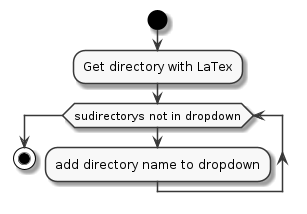
\includegraphics[width=150px]{../technical_documentation/diagramm/uml/flowcharts/gui/controller/initialiseTypeDropdown.png}
\caption{\label{initializeTypeDropdown-methode}Ablaufdiagramm der initializeTypeDropdown Methode}
\end{figure}

\begin{figure}[!htbp]
\centering
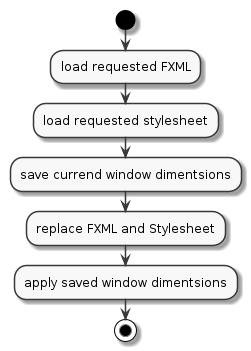
\includegraphics[width=150px]{../technical_documentation/diagramm/uml/flowcharts/gui/controller/switchToScene.png}
\caption{\label{switchToScene-methode}Ablaufdiagramm der switchToScene Methode}
\end{figure}

\subsubsection{de.thowl.aids.gui.MainScene}

\noindent Die Methode \texttt{appendToTextArea} (Abbildung~\ref{appendToTextArea-methode}) fügt eine Textzeile in eine TextArea ein, welche als Statusindikator genutzt wird.

Dazu wird der bestehende Text kopiert, der neue String angefügt, und anschließend der alte durch den neuen Text ersetzt.

\begin{figure}[!htbp]
\centering
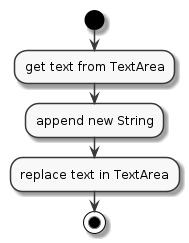
\includegraphics[width=150px]{../technical_documentation/diagramm/uml/flowcharts/gui/mainscene/appendToTextArea.png}
\caption{\label{appendToTextArea-methode}Ablaufdiagramm der sappendToTextArea Methode}
\end{figure}

\clearpage

\section{Gesprächsprokolle}

\noindent Im Folgenden werden nur die Gespräche mit den Dozenten aufgeführt,
Alles Weitere wurde bei Bedarf auf WhatsApp geklärt.

\subsection{1ste Besprechung}

\noindent Es wurden unsere Ideen und Ansätze bezüglich des Projektes vorgestellt,
und der Meilensteinplan präsentiert.
Diese wurden alle gut aufgenommen.
Im Abschluss wurde noch ein Themenwunsch für eine evtl. Vorlesung vorgeschlagen: JavaFx.

\subsection{2te Besprechung}

\noindent Es wurde der aktuelle Fortschritt bezüglich des Projektes, sowie Probleme vorgestellt.
Probleme mit den Unit-Tests konnten nach einem Vorschlag ignoriert werden (diese werden daher auch nicht weiter erwähnt).

\clearpage

\section{Implementierung (Probleme und Lösungen)}

\subsection{pdflatex}

\noindent Beim Testen der \texttt{compile()} Methode passierte absolut gar nichts15Es wurden keine Fehler oder vergleichbares ausgegeben, und von einem PDF-Dokument fehlte jede Spur.
Es gab also keinen Hinweis darauf, dass \texttt{pdflatex} ausgeführt wurde.

Um dem Ursprung auf den Grund zu gehen, sollte erstmal dafür gesorgt werden,
dass der gewohnte Output von pdflatex von unserem Programm ausgegeben wird, um Fehler erkennen zu können.
Bei der Umsetzung wurde festgestellt, dass der fehlende Output an sich die Ursache war, und eben dieser nicht blockiert werden darf.
Dieses Problem hat sich mehr oder weniger von selbst gelöst.

Um \texttt{pdflatex} auszuführen, setzten wir den Befehl als String zusammensetzen und übergaben ihn an einen Processrunnner.
Diese Art und Weise wurde plötzlich als deprecated markiert.

Nach einem Blick in die Dokumentation wurde klar, dass ein \texttt{String[]} vorgesehen ist.
Unser Ansatz sollte durch häufigen Missbrauch (nicht näher beschrieben) aus Java entfernt werden.
Der entsprechende Quellcode wurde stante pede angepasst.

\subsection{CSS-stylesheet}

\noindent Einige Elemente wie die Icons in der Seitenleiste und die Text-Area,
wollten sich nicht den in der Größe anzeigen lassen, die ursprünglich vorgesehen war.

Etwas Nachforschung ergab, dass die Icons einige Extraregeln für die Skalierung benötigten.
Da die Text-Area nach ewigen Trial-and-Error immer noch nicht die geplanten Dimensionen aufwies,
und die optische Schönheit aus Zeitgründen nicht priorisiert wurde, wurde dies als ``Designentscheidung'' angesehen und so belassen.

\subsection{ChatGPT}

\noindent ChatGPT ist bei der Beantwortung von Anfragen immer übermäßig gesprächig,
Eine typische ChatGPT-Antwort sieht in etwa so aus:

\begin{quote}
[Beschreibung der eigenen Frage] \\[0pt]
[Tatsächliche Antwort] \\[0pt]
[Kurzes Fazit, oder ähnliches] \\[0pt]
\end{quote}

\noindent Da ChatGPT durch einen Bug bei zu vielen ähnlichen Fragen in einen Zustand wechselt, indem die eigenen Rahmenbedingungen ignoriert werden, gibt es selbst mit Überredungsversuchen keine zuverlässige Möglichkeit, den für uns wichtigen Teil der Antwort zu isolieren.
Diese Feature umzusetzen würde sich als sehr schwierig erweisen, und vermutlich in kryptischen, unwartbaren regex Masken ausarten.

Das Feature wurde verworfen, es war ohnehin nur als optionale Anforderung geplant.
\end{document}
